\chapter{音声合成と音声\ruby{認識}{にん|しき}}
\section{音声合成}
音声合成とは何でしょう。それは、人間の声を人工的に機械で作り出すことです。みなさんが目にするもので言えば、例えばソフトバンクが\ruby{制作}{せい|さく}するpepper(図\ref{pepper})というロボットがあります。

\begin{figure}[H]
\begin{center}
    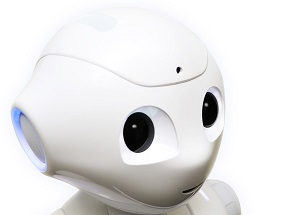
\includegraphics[width=0.5\linewidth]{images/chap06/text06-img001.jpg}
    \caption{pepper (softbank)}
    \label{pepper}
\end{center}
\end{figure}

これは声を出して利用者とコミュニケーションを取ります。pepperから声が出るのは、中に人間が入っているわけではありません。読み上げたい文章があったとき、それにマッチした音声を生成し、スピーカーから発しているのです。
今回は音声を合成するために、OpenJTalkと\ruby{呼}{よ}ばれる音声合成のためのソフトウェアを使います。OpenJTalkは、読み上げたい文章と、ひらがなごとの音(\ruby{厳密}{げん|みつ}にはもう少し多種の音)を入力し、対\ruby{応}{おう}する音声ファイルを出力します(図\ref{OpenJTalkの入出力})。

\begin{figure}[H]
\begin{center}
    \includesvg[width=\linewidth]{images/chap06/text06-img011.svg}
    \caption{OpenJTalkの入出力}
    \label{OpenJTalkの入出力}
\end{center}
\end{figure}

\begin{tcolorbox}[title=\useOmetoi]
\begin{enumerate}
        \addquiz{音声合成とはなんですか。20字以内で説明してください。}
        \addquiz{音声合成をするにはパソコンに何を\ruby{準備}{じゅん|び}する必要がありますか。3つ挙げてください。}
\end{enumerate}
\end{tcolorbox}
